\documentclass[10pt,twocolumn]{article}
	
\usepackage{myfontstyle}
\usepackage{mypackages}
\usepackage{mymacros}
\usepackage{mycommands}
\usepackage{graphicx}
\usepackage{hyperref}

\begin{document}
\thispagestyle{fancy1}

%%% Title and Abstract------------------------
\twocolumn[
\begin{center}
	\hrule
	\vspace{3pt}
	% Title:
	{\sffamily\bfseries\Large
		Report for Assignment 7: Picking-Time Neural Network
	} \\
	{\color{gray}
		\vspace{3pt}
		\hrule
		\vspace{3pt}
	}
	{
		\hspace*{\fill}
		Julian Soh
		\hspace*{\fill}
%		Second Author
%		\hspace*{\fill}
%		Third Author
%		\hspace*{\fill}
%		Fourth Author    % uncomment these two lines if there's a fourth author
%		\hspace*{\fill}
	}\\
	\vspace{3pt}
	{\itshape
		\hspace*{\fill}
		Department of Mechanical Engineering, Saint Martin's University
		\hspace*{\fill} \\
		\hspace*{\fill}
		ME/EE 467---Machine Intelligence
		\hspace*{\fill}
	}\\
	\vspace{3pt}
	{
		\hspace*{\fill}
		\today{} % today's date ... can type manually instead
		\hspace*{\fill}
	}
	\vspace{3pt}
	{\color{gray}\hrule}
%	\vspace{2pt}
\end{center}
% Abstract:
\begin{adjustwidth}{1.5in}{1.5in}
{\small
\noindent\textbf{Abstract.} \hspace{1em}
Build and train a feedforward neural network in PyTorch to predict warehouse picking times from operational features. The dataset contains nonlinear interactions that a linear model cannot capture; the exercise demonstrates when and why neural networks outperform linear models.
}
\end{adjustwidth}
\vspace{9pt}
\hrule
\vspace{1\baselineskip}
]

%%% Body -------------------------

\section{Introduction} 
\label{sec:introduction}

Linear models cannot learn non-linear data patterns. In contrast, feedforward neural networks can learn non-linear relationships between features and targets. This report demonstrates the superiority of feedforward neural networks over linear models in predicting warehouse picking times from operational features. 

A dataset containing non-linear interactions is generated. This dataset contains patterns that a linear model cannot capture, while a feedforward neural network can learn these complex relationships and make accurate predictions.

\section{Methods}

\subsection{Training Methodology}
We used a 5-fold cross-validation approach. We held 20\% of the data as a validation set and trained the model on the remaining 80\%. This process was repeated 5 times, with each fold serving as the validation set once. The training was performed for 200 epochs per fold, and the average validation loss across all folds was computed to evaluate model performance.

After cross-validation, we retrained on the full CV pool (all 5 folds combined) with the same hyperparameters and evaluated the final RMSE.

\subsection{Linear Regression Baseline}

Using Linear Regression, we used the same normalized data as the neural network. This will serve as our baseline and to compare its performance to the neural network.

\section{Results and Discussion}
\label{sec:results}

\subsection{Cross-Validation Loss Curves}
\begin{figure}[htb]
	\centering
	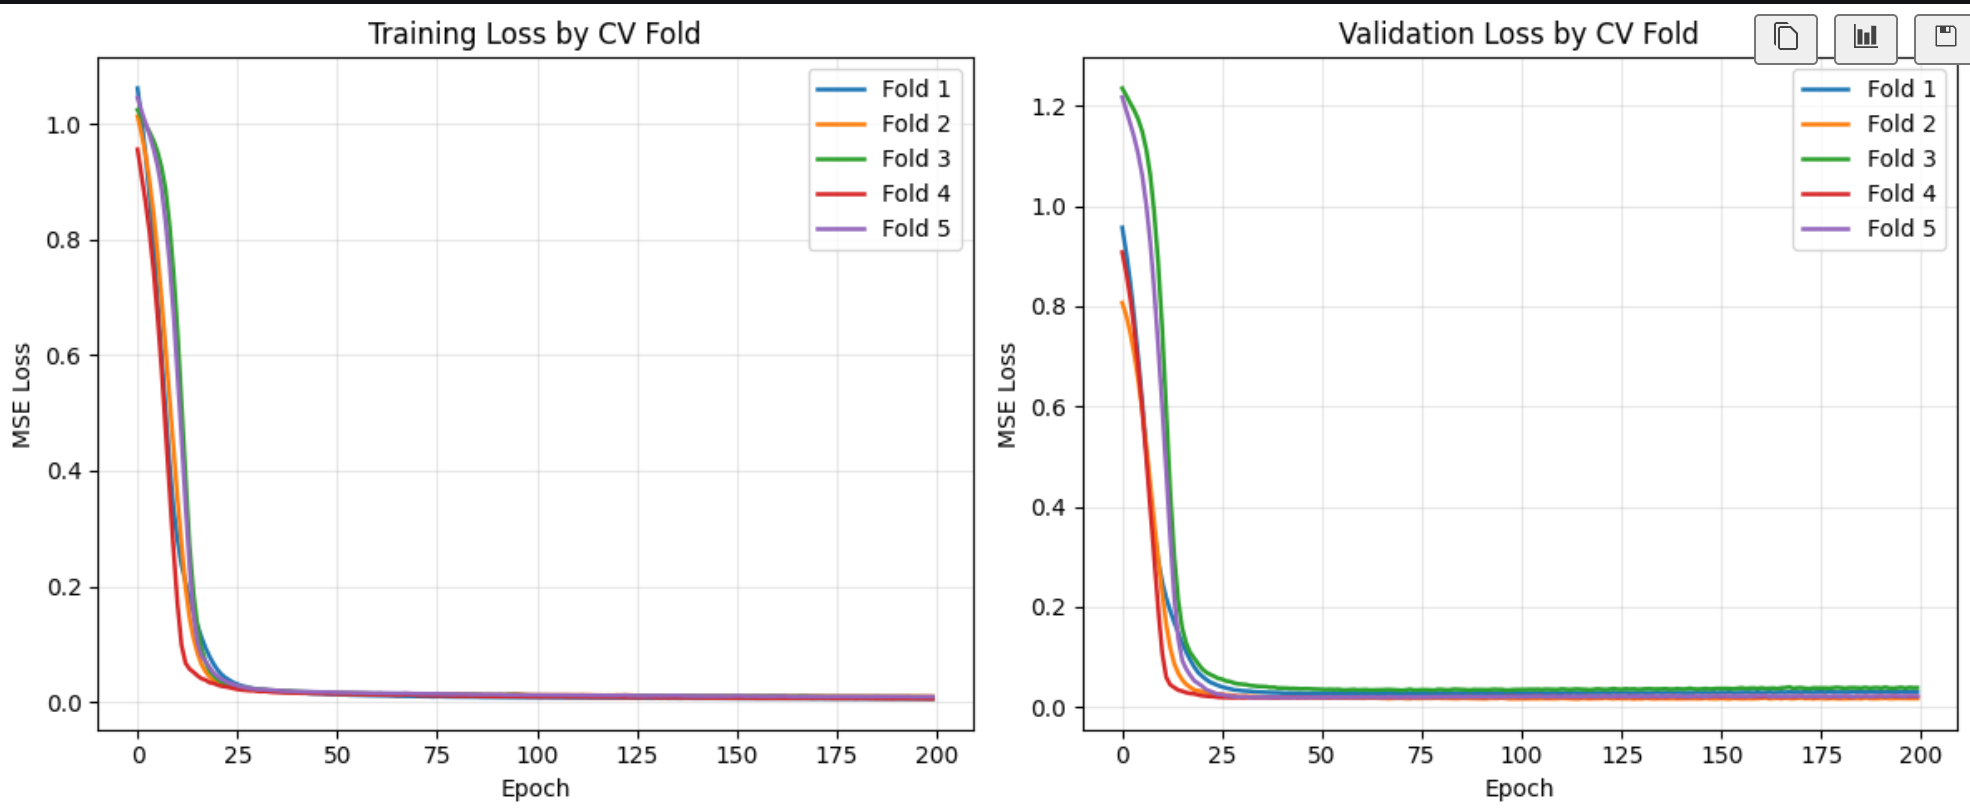
\includegraphics[width=.9\linewidth]{figures/CV_Loss_Curves.png}
	\caption{Crosss-Validation Loss Curves for 5 folds.}
	\label{fig:CV_Loss_Curves}
\end{figure}
The two plots shown in Figure \ref{fig:CV_Loss_Curves} illustrate how the neural network learns during \textbf{5-fold cross-validation}.

\begin{itemize}
  \item The \textbf{left plot} shows the \textbf{training loss} for each fold.
  \item The \textbf{right plot} shows the \textbf{validation loss} for each fold.
\end{itemize}

\textbf{Loss} measures how wrong the model is. A \textbf{lower loss} means the predictions are closer to the true picking times. Because this is a regression problem, the loss shown here is the \textbf{mean squared error (MSE)}, which penalizes larger mistakes more strongly.

Each colored line corresponds to one fold of cross-validation. In each fold, the model is trained on four subsets of the data and evaluated on the remaining held-out subset. This approach allows us to assess whether performance is consistent across different train/validation splits rather than relying on a single split.

These plots reveal several important observations:

\begin{itemize}
  \item \textbf{The loss drops very quickly in the first few epochs.}  
  This indicates that the network learns the main structure of the problem early in training.

  \item \textbf{The training loss becomes very small for all folds.}  
  This shows that the model is capable of fitting the training data well.

  \item \textbf{The validation loss also drops quickly and remains low.}  
  This is important because it suggests the model is not merely memorizing the training data, but is also performing well on unseen validation examples.

  \item \textbf{The fold-to-fold curves are similar, but not identical.}  
  This variation is expected, since each fold uses a slightly different subset of the data. The similar overall shapes of the curves suggest consistent model behavior across splits.

  \item \textbf{There is no strong evidence of overfitting.}  
  If overfitting were severe, the training loss would continue to decrease while the validation loss would increase or remain substantially higher. Instead, the validation loss stabilizes at a low level after the initial decrease.
\end{itemize}

Overall, these results indicate that the neural network trains stably, converges quickly, and generalizes well across the different cross-validation folds. This interpretation is consistent with the reported cross-validation RMSE values, which are relatively stable from fold to fold.

\subsection{Predicted versus Actual}

The two plots in \autoref{fig:Predicted_vs_Actual} illustrate the same concept for two different models. For each test example, the horizontal axis represents the \textbf{actual picking time}, while the vertical axis represents the model’s \textbf{predicted picking time}.

The dashed diagonal line corresponds to \textbf{perfect predictions}. A point lying exactly on this line indicates that the model predicted the picking time correctly. The farther a point deviates from the diagonal, the larger the prediction error.

The plot for the \textbf{linear model} shows a clear overall trend, indicating that the model has learned some useful structure in the data. As the actual picking time increases, the predicted picking time also tends to increase. However, many points lie farther from the diagonal, particularly at the lower and higher ends of the range. This indicates that while the linear model captures the general direction of the relationship, it fails to model the full shape of the underlying function accurately.

A particularly important feature of the linear model plot is the presence of \textbf{systematic errors} rather than purely random noise. For larger actual picking times, many points fall \textbf{below} the diagonal, indicating that the model is consistently \textbf{under-predicting} slow or difficult cases. In other words, as task complexity increases, the linear model tends to produce predictions that are too low. This behavior is consistent with the fact that the true data-generating process includes nonlinear effects that a simple linear model cannot represent.

The plot for the \textbf{neural network} is noticeably tighter around the diagonal. This indicates that its predictions are generally closer to the true values. Although the points do not lie perfectly on the diagonal—due to noise in the data and the inherent limitations of any model—the overall scatter is reduced compared to the linear model. As a result, the neural network produces smaller prediction errors on average.

The improvement offered by the neural network is most apparent in regions where the linear model struggles:

\begin{itemize}
  \item \textbf{At higher picking times}, the neural network remains closer to the diagonal, indicating better handling of more difficult cases.
  \item \textbf{At the extremes of the range}, the neural network exhibits less systematic bias than the linear model.
  \item \textbf{Across the middle range}, both models perform reasonably well, but the neural network remains more tightly clustered around the ideal prediction line.
\end{itemize}

In plain terms, this comparison shows that while the linear model captures the broad trend in the data, it is too limited to represent interaction effects, threshold behaviors, and curvature. The neural network, by contrast, is better able to model these nonlinear patterns, resulting in predictions that align more closely with the actual outcomes.

This visual assessment is consistent with the quantitative results: the neural network achieves a lower RMSE than the linear model. Thus, the improved scatter plot is not merely cosmetic, but reflects genuinely superior predictive accuracy.
\begin{figure}
	\centering
	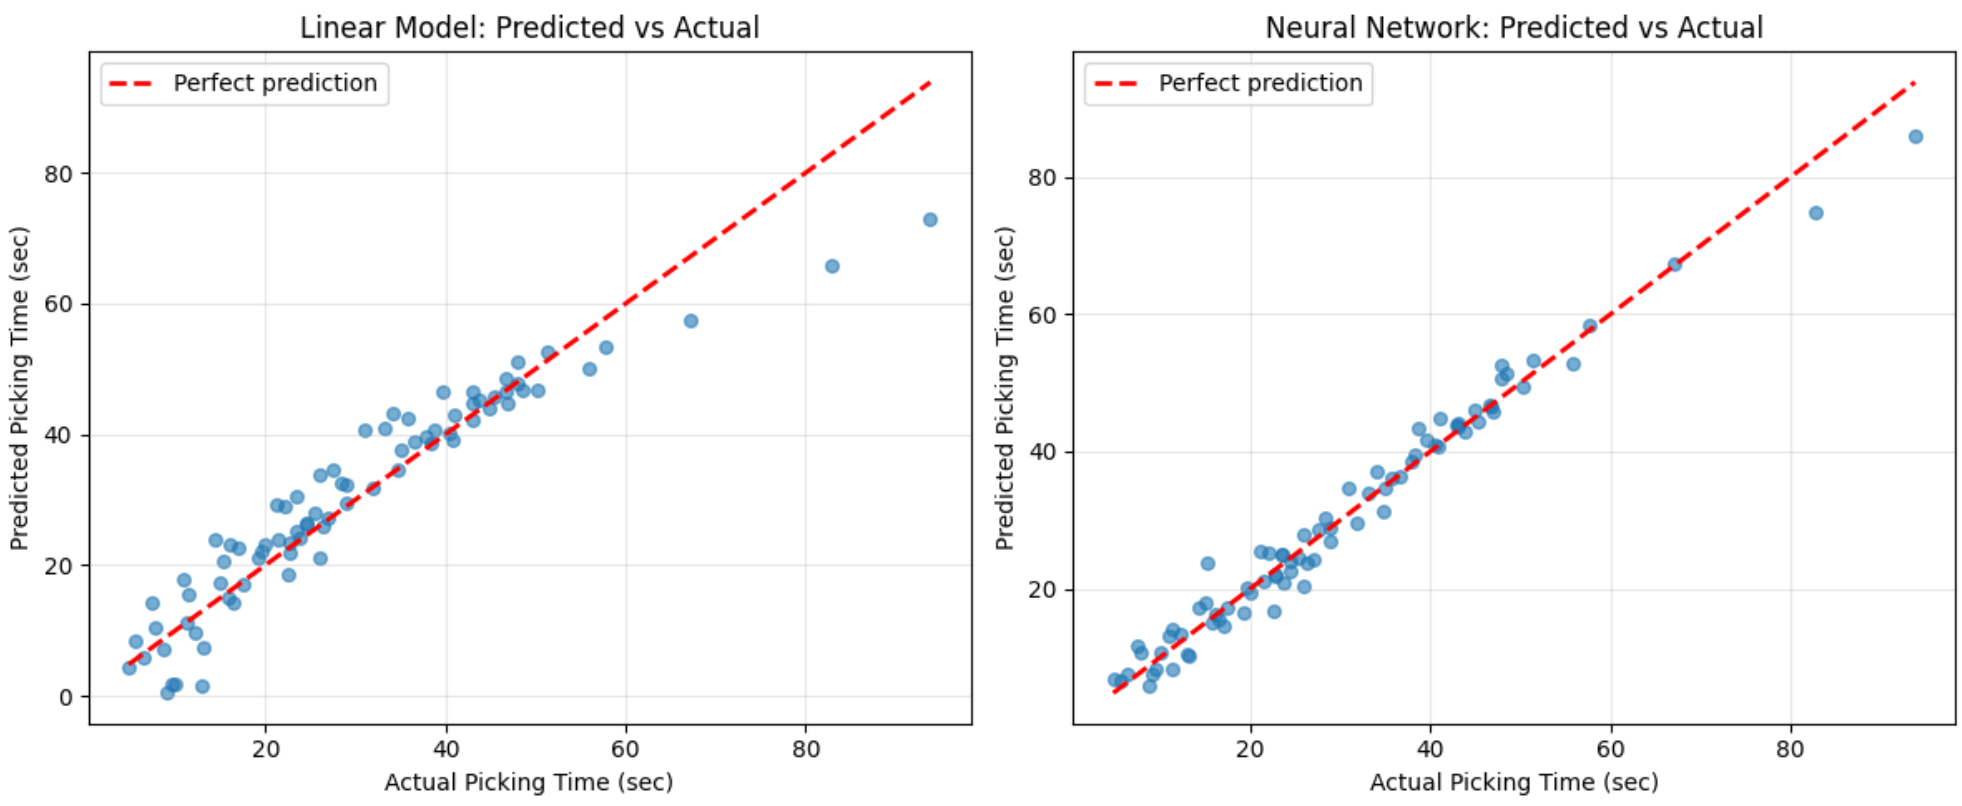
\includegraphics[width=.9\linewidth]{figures/Predicted_vs_Actual_curves.png}
	\caption{Predicted vs Actual picking times for the final model.}
	\label{fig:Predicted_vs_Actual}
\end{figure}

\begin{table}[h]
\centering
\begin{tabular}{lccc}
\hline
\textbf{Model} & \textbf{Test RMSE (sec)} & \textbf{Relative to Linear} & \textbf{RMSE Improvement (\%)} \\
\hline
Linear Regression & 5.45 & 1.000 & 0.00 \\
Neural Network    & 2.72 & 0.499 & 50.12 \\
\hline
\end{tabular}
\caption{Test RMSE comparison between linear regression and neural network models.}
\label{tab:rmse_comparison}
\end{table}
The \textbf{linear-vs.-neural network RMSE comparison} confirms the visual results (\autoref{fig:Predicted_vs_Actual}) quantitatively, the neural network achieves a lower test RMSE than ordinary least squares.

This outcome is expected because the linear baseline can only learn an \emph{affine} relationship in the original input space. In contrast, a multilayer neural network can represent nonlinear functions through compositions of linear transformations and nonlinear activation functions.

\subsection{Depth Experiment Curves}
The \textbf{depth experiment curves} shown in \autoref{fig:Depth_Experiment_Curves} add a more detailed picture. 
The mean validation-loss curves for 1, 2, and 3 hidden layers show how model depth affects optimization and validation behavior over training epochs. 

In the accompanying Jupyter notebook with the experiment, we see that deeper models do not automatically guarantee better
performance; instead, the experiment shows that architecture choice should be validated empirically. This is consistent with the discussion that additional depth can improve expressive power, but its practical benefit depends on the task and data.
\begin{figure}
	\centering
	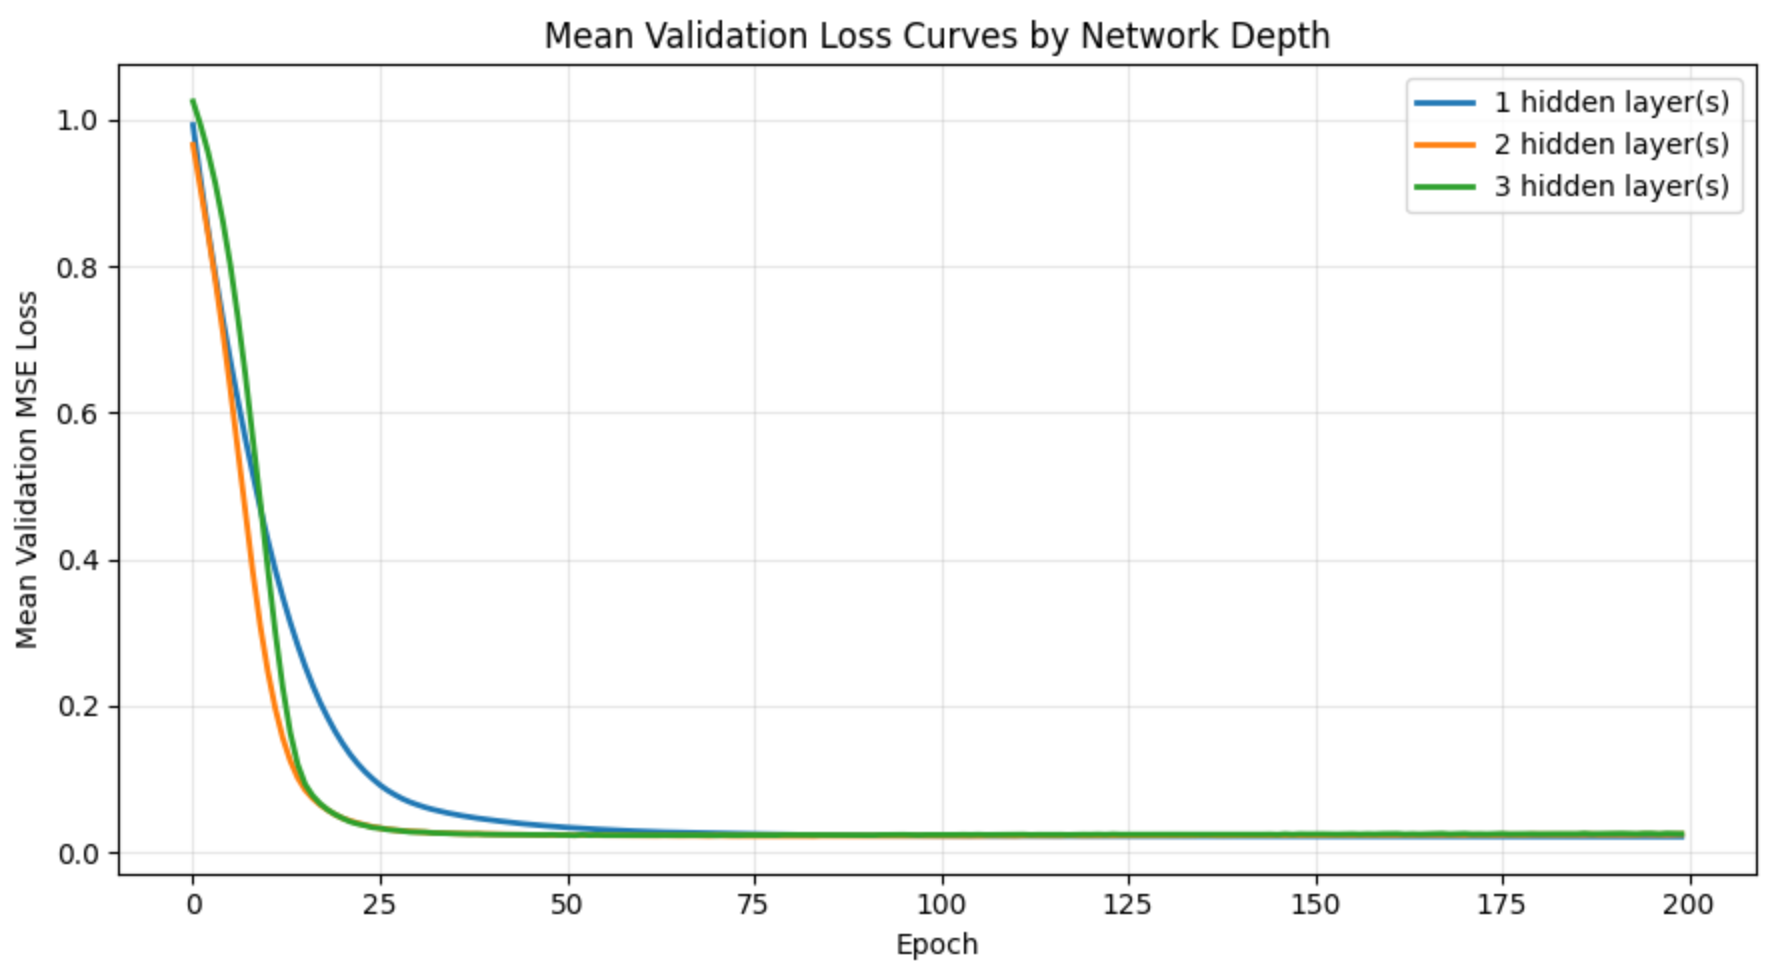
\includegraphics[width=.9\linewidth]{figures/Depth_Experiment_Curves.png}
	\caption{Test RMSE for different model depths.}
	\label{fig:Depth_Experiment_Curves}
\end{figure}

\subsection{Neural Network improvement over Linear}

The neural network improves most over the linear model in the parts of the input space where the target function is explicitly non-linear:
\begin{itemize}
	\item \textbf{High distance with high congestion}: the target includes an interaction term (`congestion * distance`), which a plain linear model cannot represent without manually engineered interaction features.
	\item \textbf{Low battery values}: the target includes a threshold-style penalty when `battery < 0.2`, which is not naturally captured by a linear model.
	\item \textbf{Larger distances}: the quadratic distance term introduces curvature, again favoring a nonlinear model.
\end{itemize}

\section{Conclusion}
Taken together, the CV loss curves, the predicted-vs.-actual scatter plots, the RMSE comparison, and the depth experiment all support the same conclusion: the neural network is better suited than linear regression for this warehouse picking-time problem because the underlying data is not purely linear.

%%% References -------------------------

\nocite{*}
\bibliographystyle{plainnat}
\bibliography{report}


%%% Appendices -------------------------

\end{document}  